\documentclass[12pt]{article}
\usepackage{graphics}

% the following is to get inch margins on a letter-size paper
\setlength{\topmargin}{0pt}
\setlength{\headheight}{0in}
\setlength{\headsep}{0in}
\setlength{\textheight}{9.0in}
\setlength{\footskip}{0.5in}
\setlength{\oddsidemargin}{0pt}
\setlength{\evensidemargin}{0pt}
\setlength{\textwidth}{6.5in}

\usepackage{algorithm,algpseudocode, hyperref}

\begin{document}

% no page numbers on this page
\thispagestyle{empty}

\begin{center}
{\Large \bf Privacy-Focused Raspberry Pi-based AI Assistant Leveraging On-Device Machine Learning}\\[3mm]

Nithun Selva, Clio Zhu\\[6mm]
\end{center}

\begin{abstract}
	With the recent advancements in artificial intelligence and machine learning, personal digital assistants are becoming more mainstream. However, these often lack a personalized touch and raise substantial privacy and ethical concerns. Our project explores developing a private and intelligent AI assistant powered by a Raspberry Pi 5. This assistant is designed to address the growing discomfort in human-robot interactions and the ethical dilemmas arising from rapid technological advancements. 

	Our primary goals include: 
	Privacy-Centric Design: Employs state-of-the-art on-device machine learning to ensure user data remains private and secure. This means no internet connection is necessary, as everything is run locally. 
	Multifunctional Capabilities: Supports translation, multilingual chatting, and image generation using locally run pre-trained large language models. 
	User-Friendly and Intuitive: Prioritizes ease of use without compromising functionality, offering a secure and personalized user experience. 
\end{abstract}

\section{Introduction}
With the recent advancements in artificial intelligence and machine learning, personal digital assistants are becoming more mainstream. However, these often lack a personalized touch and raise substantial privacy and ethical concerns. Our project explores developing a private and intelligent AI assistant powered by a Raspberry Pi 5. This assistant is designed to address the growing discomfort in human-robot interactions and the ethical dilemmas arising from rapid technological advancements. 

Our primary goals include: 
Privacy-Centric Design: Employs state-of-the-art on-device machine learning to ensure user data remains private and secure. This means no internet connection is necessary, as everything is run locally. 
Multifunctional Capabilities: Supports translation, multilingual chatting, and image generation using locally run pre-trained large language models. 
User-Friendly and Intuitive: Prioritizes ease of use without compromising functionality, offering a secure and personalized user experience. 

\subsection{Background}
Initial Surveys

As the focus of our project is deeply rooted in understanding and addressing user needs, we initiated our efforts by conducting a comprehensive survey. This survey was designed to gather detailed insights into how potential users interact with and perceive current AI technologies. 

\subsection{Architecture}

This project is programmed to be as modular as possible, both in the hardware and software. Each model is a self-contained class, which makes it quite easy to test different models. We use a Raspberry Pi 5 with a 5” round touchscreen and a microphone in a customized 3D-printed enclosure. The user interface is designed to have minimal UI elements to enhance ease of use.

Our testing phase is comprehensive, evaluating the assistant's performance in various scenarios to ensure that privacy, ease of use, accuracy, and user satisfaction are all up to our high standards. We conduct iterative tests to fine-tune the device based on user feedback and performance data, continuously refining our system to meet the needs of our users better. 

As the Pi doesn't have native hardware for accelerating ML workloads, we use a workstation in Davis with an RTX 4090 communicating with the Raspberry Pi to process tasks. This approach allowed us to  enhance performance without compromising data privacy/integrity. 

Our framework is designed around the following advanced AI models:
OpenAI Whisper: transcribing audio inputs into text, recognizing the language, and translating it when necessary.
Google Gemma (7B): classifies inputs to determine whether they are for image generation, translation, or chat. We used few-shot prompting to improve predictions. 
Mistral (7B): Generates chat/text prompt outputs. 
Meta NLLM: For language translations.
Stable Diffusion XL: For image generation tasks.

\begin{figure}[bht]
\begin{center}
{\resizebox{4in}{!}{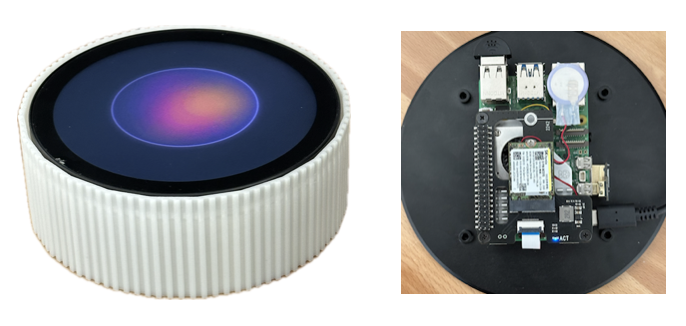
\includegraphics{device.png}}}
%        {x-dim}{y-dim}
% ! means proportional scaling
\end{center}
\vspace{-5mm} % just to remove the extra space between the figure and the
              % caption
\caption{Picture of devicet.}
\label{figurelabel}
\end{figure}

\begin{figure}[bht]
	\begin{center}
	{\resizebox{4.5in}{!}{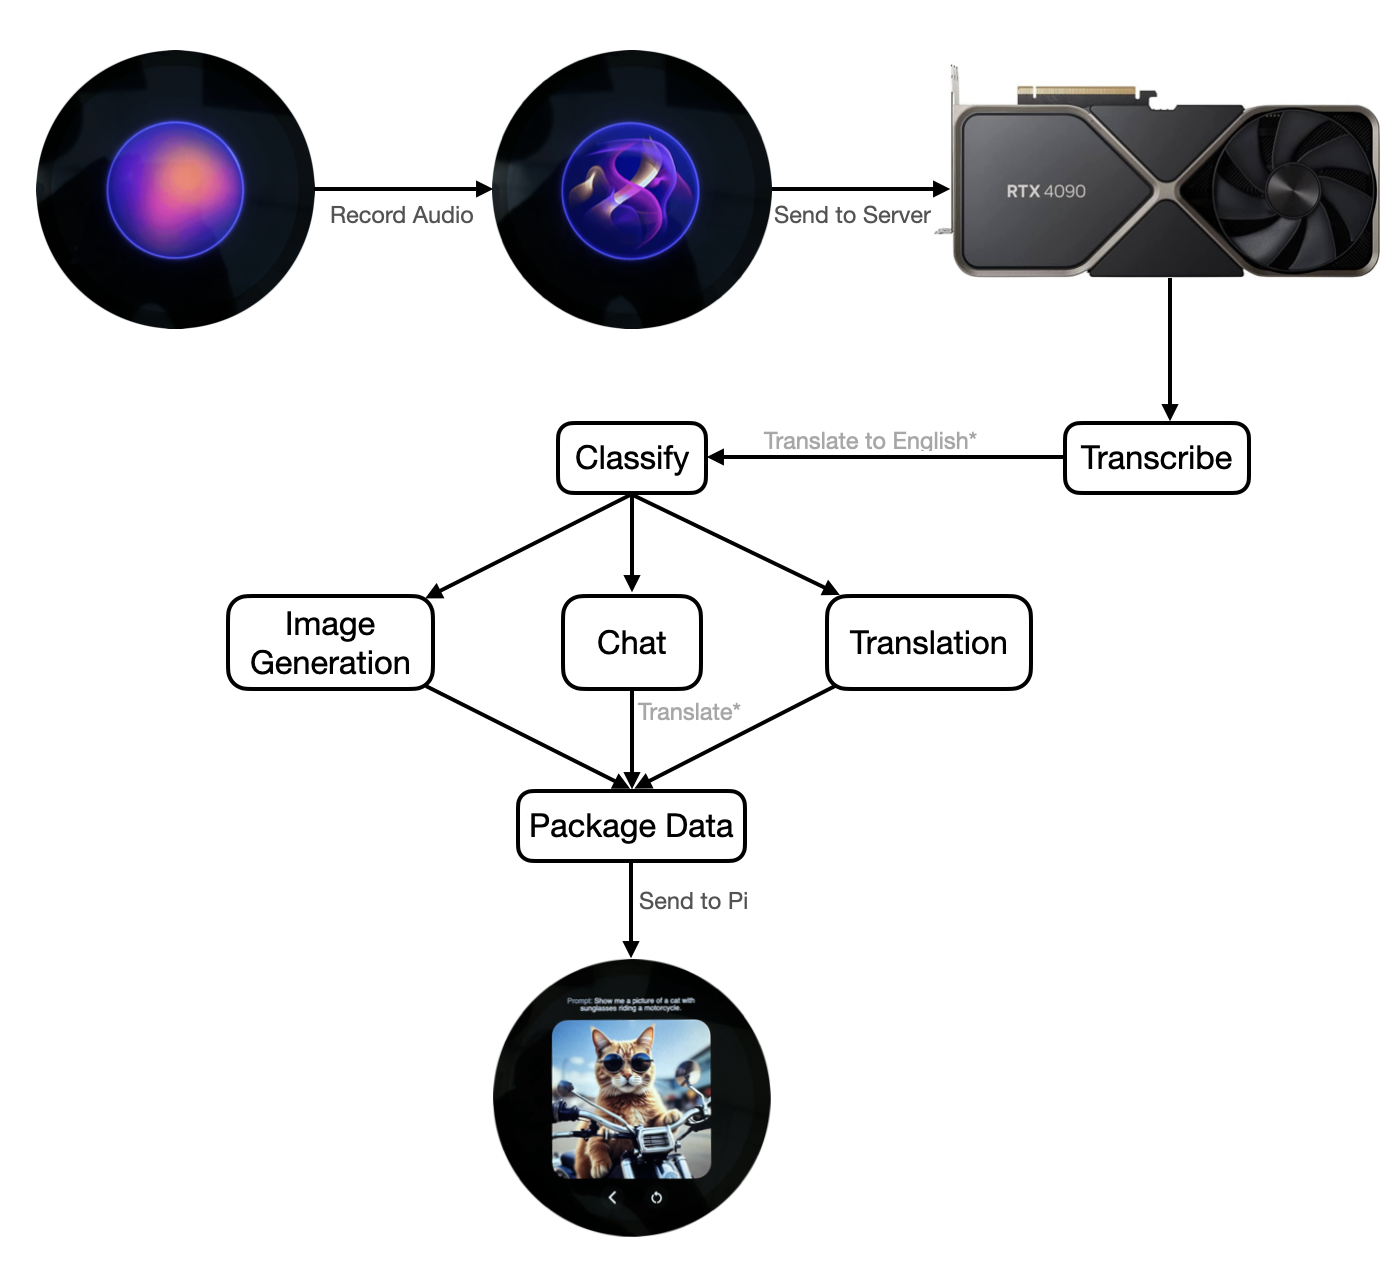
\includegraphics{chart.png}}}
	%        {x-dim}{y-dim}
	% ! means proportional scaling
	\end{center}
	\vspace{-5mm} % just to remove the extra space between the figure and the
				  % caption
	\caption{How the server works.}
	\label{figurelabel}
	\end{figure}


\begin{itemize}
\item One
\item Two
\item There
\end{itemize}

\begin{enumerate}
\item One
\item Two
\item There
\end{enumerate}

\begin{description}
\item[Item 1:] Ut enim ad minim veniam, quis nostrud exercitation ullamco
laboris nisi ut aliquip ex ea commodo consequat.
\item[Item 2:]  Duis aute irure dolor in reprehenderit in voluptate
velit esse cillum dolore eu fugiat nulla pariatur.
\item[Item 3:]  Excepteur sint occaecat cupidatat non proident, sunt in
culpa qui officia deserunt mollit anim id est laborum.

\end{description}

The correlation analysis of user satisfaction metrics underscores the importance of the structure of a response, with a significant correlation, highlighting that users value clear and logical answers the most. Speech recognition accuracy and response time also affect satisfaction, indicating that effective communication and speed are key to a positive user experience. Other features like image generation, though beneficial, are less critical to overall satisfaction.

\section{Results}

User Experience Enhancements: Users appreciated the quick responsiveness and user-friendly interface of the assistant. Improvements could include reducing distractions from background noise and updating the database more frequently.
Feature Additions: Several suggestions for new features were mentioned, such as better handling of multilingual interactions, more basic informational queries, and improvements in image generation capabilities, particularly concerning copyright issues. Future improvements could include fine tuning the models (particularly the classifier), as we are currently only running pre-trained models. 
Privacy and Trust: Given the focus on privacy it might be beneficial to include more explicit information or features that reassure users about how their data is being handled and protected. 


\section*{Acknowledgements}
We want to thank Prof.~Ying Li for her invaluable feedback and her guidance throughout this project. \\
We would also like to thank MuleWorks for help with 3D printing the enclosure for our device.

\begin{thebibliography}{1}

\bibitem{aodv}
Shin, Jong-Gyu, Ga-Young Choi, Han-Jeong Hwang, and Sang-Ho Kim (2021), ``\emph{Evaluation of Emotional Satisfaction Using Questionnaires in Voice-Based Human-AI Interaction},'' Applied Sciences 11, no. 4: 1920. \href{https://doi.org/10.3390/app11041920}{https://doi.org/10.3390/app11041920}

\bibitem{aodv}
Carmody, J., Shringarpure, S. and Van de Venter, G. (2021), ``\emph{AI and privacy concerns: a smart meter case study},'' Journal of Information, Communication and Ethics in Society, Vol. 19 No. 4, pp. 492--505. \href{https://doi.org/10.1108/JICES-04-2021-0042}{https://doi.org/10.1108/JICES-04-2021-0042}
% add urls hyperlinks to the references 

\end{thebibliography}

\end{document}
